\documentclass[10pt, aspectratio=169]{beamer}

\usetheme{Madrid}
\usecolortheme{default}
\setbeamertemplate{navigation symbols}{}
\setbeamertemplate{footline}{%
  \hfill\insertframenumber/\inserttotalframenumber\hspace*{4pt}\vspace{2pt}}

\usepackage{booktabs}
\usepackage{multirow}
\usepackage{graphicx}
\usepackage{xspace}
\usepackage{adjustbox}
\usepackage{tikz}
\usetikzlibrary{positioning, arrows.meta, fit, calc}

\graphicspath{{../../figures/}}

\title{Mini Colossal-AI: Distributed Parallelism from Scratch}
\subtitle{Phase 3 --- Communication-Aware Placement on Heterogeneous GPU Clusters}
\date{}
\author{Dinesh Chand \and Goutham P \and Meena Chidambaram \and Nadhiya R S}
\institute{MTech-AI, IISc Bangalore}

\begin{document}

% ======== TITLE ========
\begin{frame}
  \titlepage
\end{frame}

% ==================================================================
\section{Problem Statement \& Background}
% ==================================================================

% --- Slide 1: Problem Statement (Dinesh) ---
\begin{frame}{Problem Statement \& Motivation}
  \begin{itemize}
    \item Large language models (100M--billions of params) \textbf{exceed single-GPU memory}
    \item Distributed training is essential---but \textbf{which parallelism strategy} to use?
    \item Production frameworks (DeepSpeed, Colossal-AI) hide internals---hard to understand trade-offs
  \end{itemize}

  \vspace{0.8em}
  \textbf{Our goal:} Build every parallelism strategy \emph{from scratch} using only \texttt{torch.distributed} primitives, and study how \textbf{hardware topology} affects their relative performance.

  \vspace{0.5em}
  \begin{block}{Mini Colossal-AI --- Four Strategies from Scratch}
    \small
    \textbf{Data Parallelism (DP):} replicate model, sync gradients \quad
    \textbf{ZeRO:} shard optimizer states \\
    \textbf{Tensor Parallelism (TP):} split layers, 2 all-reduces/block \quad
    \textbf{Pipeline Parallelism (PP):} split stages, send activations
  \end{block}
\end{frame}

% --- Slide 2: Phase 2 Recap + Phase 3 Questions (Dinesh) ---
\begin{frame}{Phase 2 Recap \& Phase 3 Questions}
  \begin{columns}[T]
  \begin{column}{0.52\textwidth}
    \textbf{Phase 2:} 4$\times$ g4dn.xlarge, 1 T4/node, \textbf{all TCP}
    \vspace{0.2em}

    \centering
    \small
    \begin{tabular}{lrr}
      \toprule
      \textbf{Strategy} & \textbf{tok/s} & \textbf{Mem} \\
      \midrule
      Single GPU & 1,361 & 7.67 GB \\
      DP (NCCL) & 1,393 & 7.67 GB \\
      TP (4-way) & 959 & 3.38 GB \\
      PP 1F1B & 3,070 & 2.56 GB \\
      DP2$\times$PP2 & 2,281 & 4.08 GB \\
      \bottomrule
    \end{tabular}

    \vspace{0.3em}
    \raggedright
    \small PP dominated; TP/DP bottlenecked by slow TCP.
  \end{column}
  \begin{column}{0.45\textwidth}
    \textbf{Phase 3 Research Questions:}
    \begin{enumerate}
      \item How does \textbf{PCIe vs.\ TCP} change strategy ranking?
      \item Can \textbf{communication-aware placement} unlock 3D hybrid throughput?
      \item Do trends hold across \textbf{architectures}?
    \end{enumerate}

    \vspace{0.5em}
    \small
    \textit{Faculty feedback:} ``Experiments with more models showing similar trends should be done.''

    \vspace{0.3em}
    $\Rightarrow$ Add \textbf{T5-base} (encoder-decoder) alongside GPT-2 (decoder-only).
  \end{column}
  \end{columns}
\end{frame}

% ==================================================================
\section{Methodology}
% ==================================================================

% --- Slide 3: Hardware Setup (Goutham) ---
\begin{frame}{Hardware: Phase 2 $\rightarrow$ Phase 3}
  \centering
  \adjustbox{max width=\textwidth}{%
  \begin{tabular}{lll}
    \toprule
    & \textbf{Phase 2: g4dn.xlarge} & \textbf{Phase 3: g4dn.12xlarge} \\
    \midrule
    \textbf{Nodes} & 4 & 2 \\
    \textbf{GPUs / node} & 1$\times$ T4 (16 GB) & 4$\times$ T4 (16 GB each) \\
    \textbf{Total GPUs} & 4 & 8 \\
    \textbf{Intra-node} & N/A (1 GPU/node) & PCIe ($\sim$15 GB/s) \\
    \textbf{Inter-node} & TCP ($\sim$0.6 GB/s) & TCP ($\sim$0.6 GB/s) \\
    \bottomrule
  \end{tabular}}

  \vspace{0.8em}
  Phase 3 has a \textbf{mixed-speed topology}: fast PCIe within each node, slow TCP between nodes.

  \vspace{0.2em}
  \textbf{25$\times$ bandwidth gap} $\Rightarrow$ enables communication-aware placement.
\end{frame}

% --- Slide 4: Communication-Aware Placement (Goutham) ---
\begin{frame}{Communication-Aware Placement}
  \begin{columns}[T]
  \begin{column}{0.45\textwidth}
    Place the \textbf{heaviest} axis on the \textbf{fastest} link:

    \vspace{0.5em}
    \small
    \begin{tabular}{lll}
      \toprule
      \textbf{Placement} & \textbf{Inter-node} & \textbf{Intra-node} \\
      \midrule
      Good & PP & DP + TP \\
      TP inter & TP & DP + PP \\
      Bad & DP & PP + TP \\
      \bottomrule
    \end{tabular}

    \vspace{0.5em}
    Full 3D mesh: \textbf{DP=2 $\times$ PP=2 $\times$ TP=2}

    \vspace{0.3em}
    \small No code changes---only reorder mesh axes in the unified 3D plugin.
  \end{column}
  \begin{column}{0.52\textwidth}
    \centering
    \resizebox{\textwidth}{!}{%
    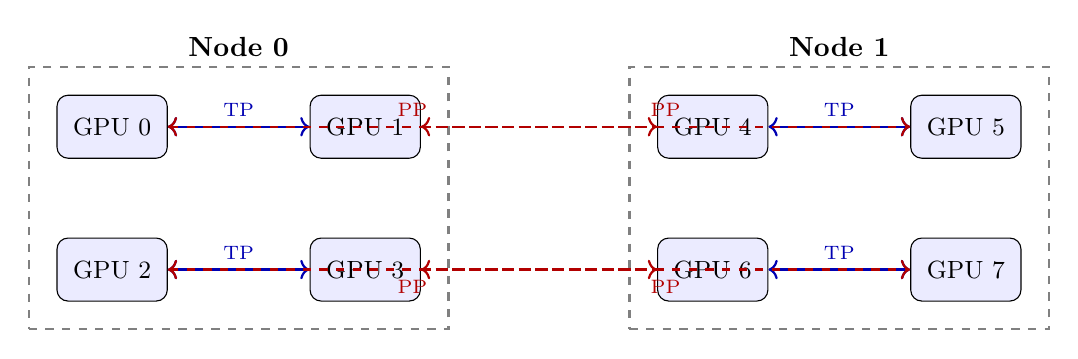
\begin{tikzpicture}[
      gpu/.style={draw, rounded corners, minimum width=1.4cm, minimum height=0.8cm, font=\small, fill=blue!8},
      pcie/.style={<->, thick, blue!70!black},
      tcp/.style={<->, thick, red!70!black, dashed},
      node distance=1cm and 1.8cm
    ]
      \node[gpu] (g0) {GPU 0};
      \node[gpu, right=of g0] (g1) {GPU 1};
      \node[gpu, below=of g0] (g2) {GPU 2};
      \node[gpu, right=of g2] (g3) {GPU 3};
      \node[draw, dashed, gray, thick, fit=(g0)(g1)(g2)(g3), inner sep=10pt, label=above:{\textbf{Node 0}}] {};

      \node[gpu, right=3cm of g1] (g4) {GPU 4};
      \node[gpu, right=of g4] (g5) {GPU 5};
      \node[gpu, below=of g4] (g6) {GPU 6};
      \node[gpu, right=of g6] (g7) {GPU 7};
      \node[draw, dashed, gray, thick, fit=(g4)(g5)(g6)(g7), inner sep=10pt, label=above:{\textbf{Node 1}}] {};

      \draw[pcie] (g0) -- (g1) node[midway, above, font=\scriptsize, blue!70!black] {TP};
      \draw[pcie] (g2) -- (g3) node[midway, above, font=\scriptsize, blue!70!black] {TP};
      \draw[pcie] (g4) -- (g5) node[midway, above, font=\scriptsize, blue!70!black] {TP};
      \draw[pcie] (g6) -- (g7) node[midway, above, font=\scriptsize, blue!70!black] {TP};

      \draw[tcp] (g0) -- (g4) node[midway, above, font=\scriptsize, red!70!black] {PP};
      \draw[tcp] (g1) -- (g5) node[midway, above, font=\scriptsize, red!70!black] {PP};
      \draw[tcp] (g2) -- (g6) node[midway, below, font=\scriptsize, red!70!black] {PP};
      \draw[tcp] (g3) -- (g7) node[midway, below, font=\scriptsize, red!70!black] {PP};
    \end{tikzpicture}}

    \vspace{0.2em}
    \scriptsize
    \textcolor{blue!70!black}{\textbf{Blue:}} TP on PCIe \quad
    \textcolor{red!70!black}{\textbf{Red dashed:}} PP on TCP
  \end{column}
  \end{columns}
\end{frame}

% --- Slide 5: PCIe vs TCP (Goutham) ---
\begin{frame}{PCIe vs.\ TCP: Why Placement Matters}
  \begin{columns}
  \begin{column}{0.55\textwidth}
    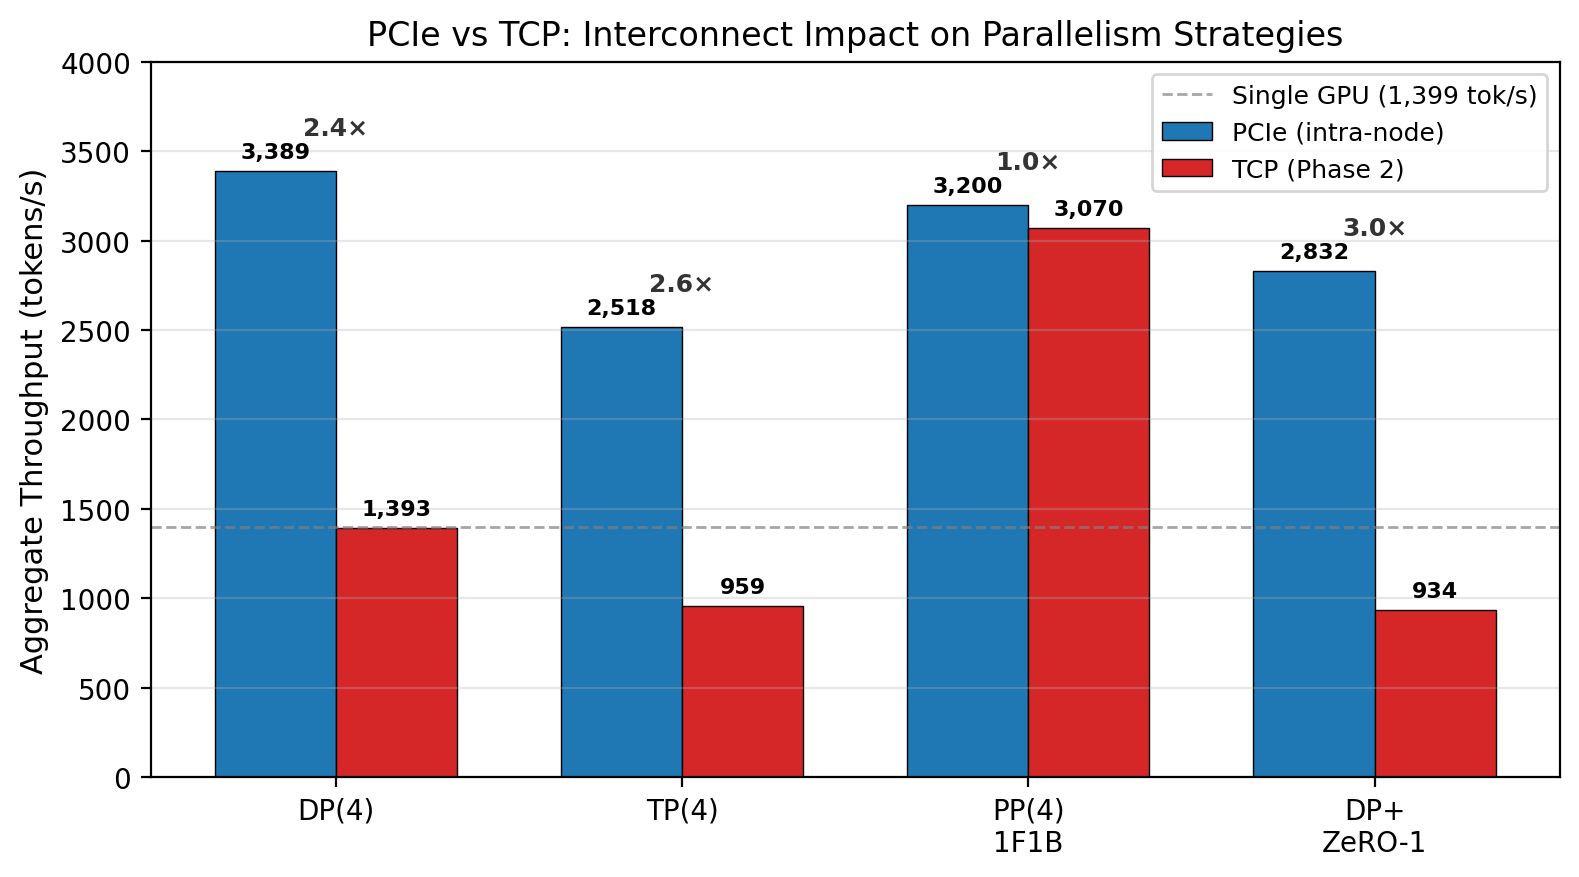
\includegraphics[width=\textwidth]{fig_phase3_pcie_vs_tcp.png}
  \end{column}
  \begin{column}{0.42\textwidth}
    \small
    \textbf{Single-node PCIe vs.\ Phase 2 TCP:}

    \vspace{0.3em}
    \begin{tabular}{lrr}
      \toprule
      \textbf{Strategy} & \textbf{PCIe} & \textbf{vs TCP} \\
      \midrule
      DP(4) & 3,389 & 2.4$\times$ \\
      TP(4) & 2,518 & 2.6$\times$ \\
      PP(4) 1F1B & 3,200 & 1.04$\times$ \\
      ZeRO-1 & 2,832 & 3.0$\times$ \\
      \bottomrule
    \end{tabular}

    \vspace{0.5em}
    DP and TP \textbf{need} fast links (2.4--3$\times$).

    PP \textbf{tolerates} slow links (1.04$\times$).

    \vspace{0.3em}
    $\Rightarrow$ Put PP on TCP, keep DP+TP on PCIe.
  \end{column}
  \end{columns}
\end{frame}

% ==================================================================
\section{Placement Results}
% ==================================================================

% --- Slide 6: Good vs Bad (Meena) ---
\begin{frame}{Good vs.\ Bad Placement --- GPT-2 Medium (8 GPUs)}
  \begin{columns}
  \begin{column}{0.50\textwidth}
    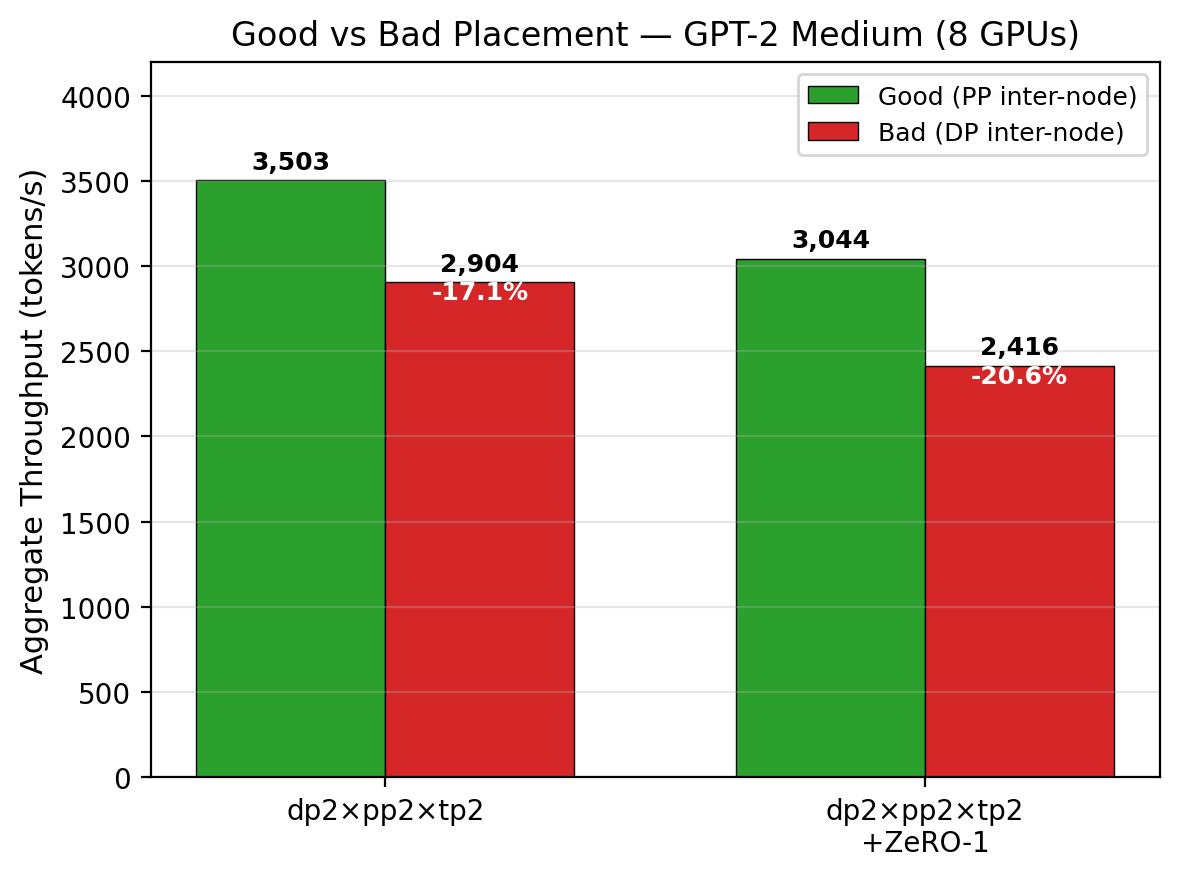
\includegraphics[width=\textwidth]{fig_phase3_good_vs_bad.png}
  \end{column}
  \begin{column}{0.47\textwidth}
    \small
    \textbf{dp=2, pp=2, tp=2:}

    \vspace{0.3em}
    \begin{tabular}{lrrr}
      \toprule
      \textbf{Config} & \textbf{Good} & \textbf{Bad} & \textbf{$\Delta$} \\
      \midrule
      Base & 3,503 & 2,904 & $-$17\% \\
      +ZeRO-1 & 3,044 & 2,416 & $-$21\% \\
      \bottomrule
    \end{tabular}

    \vspace{0.5em}
    Good placement is \textbf{$\sim$20\% faster}.

    \vspace{0.3em}
    ZeRO-1 \textbf{widens} the gap---extra optimizer-state communication adds to the DP axis load forced onto slow TCP.
  \end{column}
  \end{columns}
\end{frame}

% --- Slide 7: Three-Way Placement (Meena) ---
\begin{frame}{Three-Way Placement: A Surprising Finding}
  \begin{columns}
  \begin{column}{0.55\textwidth}
    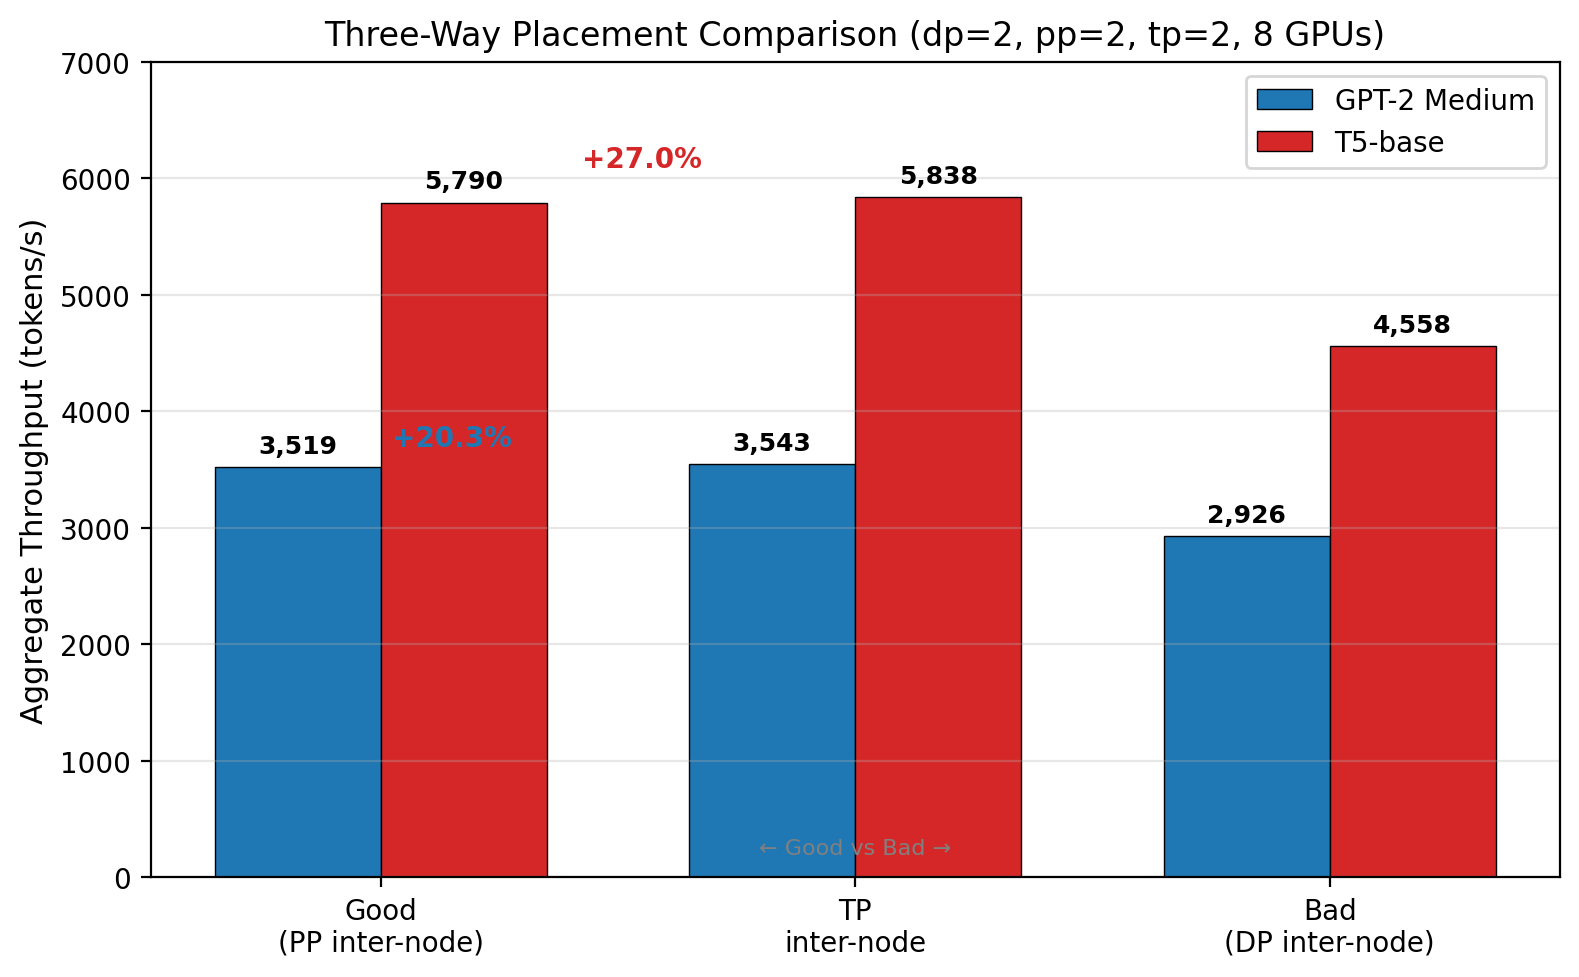
\includegraphics[width=\textwidth]{fig_phase3_three_way_placement.png}
  \end{column}
  \begin{column}{0.42\textwidth}
    \small
    \begin{tabular}{lrr}
      \toprule
      \textbf{Placement} & \textbf{GPT-2} & \textbf{T5} \\
      \midrule
      Good (PP inter) & 3,519 & 5,790 \\
      TP inter-node & 3,543 & 5,838 \\
      Bad (DP inter) & 2,926 & 4,558 \\
      \midrule
      Good vs Bad & +20\% & +27\% \\
      \bottomrule
    \end{tabular}

    \vspace{0.5em}
    \textbf{Surprise:} TP inter-node $\approx$ Good!

    \vspace{0.3em}
    At TP=2, messages are small (KB--MB).

    \textbf{DP is the real bottleneck}---it sends the \emph{entire} gradient ($\sim$1.4 GB for GPT-2, $\sim$950 MB for T5) in one shot.

    \vspace{0.3em}
    \textbf{Correct heuristic:} Keep DP on the fastest link.
  \end{column}
  \end{columns}
\end{frame}

% --- Slide 8: Multi-Model GPT-2 (Meena) ---
\begin{frame}{Multi-Model GPT-2 Placement (8 GPUs)}
  \begin{columns}
  \begin{column}{0.55\textwidth}
    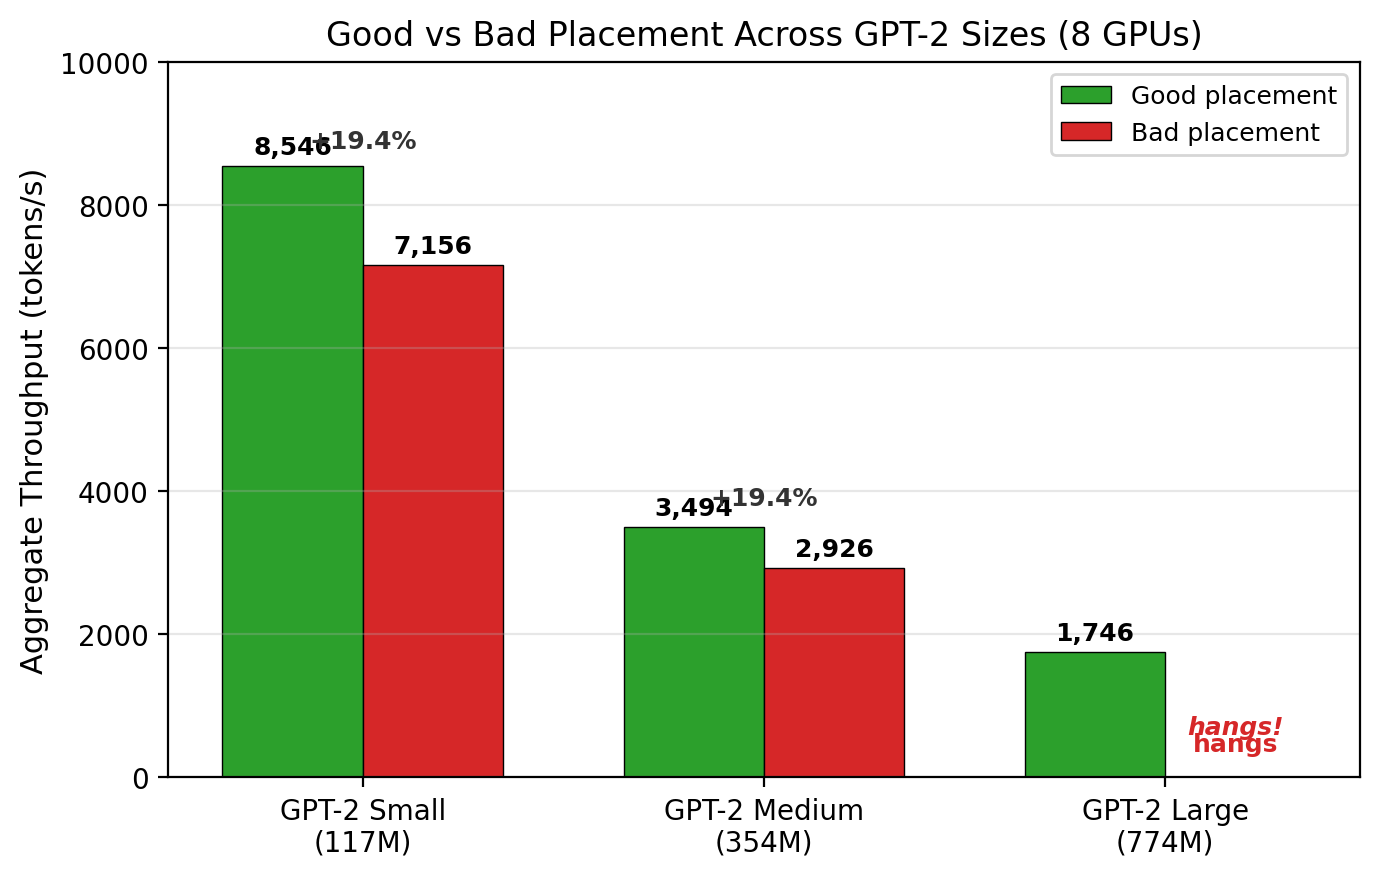
\includegraphics[width=\textwidth]{fig_phase3_multimodel_placement.png}
  \end{column}
  \begin{column}{0.42\textwidth}
    \small
    \begin{tabular}{lrr}
      \toprule
      \textbf{Model} & \textbf{Good} & \textbf{Bad} \\
      \midrule
      Small (117M) & 8,546 & 7,156 \\
      Medium (354M) & 3,494 & 2,926 \\
      Large (774M) & 1,746 & \textit{hangs} \\
      \bottomrule
    \end{tabular}

    \vspace{0.5em}
    Good placement wins \textbf{consistently} ($\sim$19--20\% faster across all sizes).

    \vspace{0.3em}
    GPT-2 Large \textbf{hangs} under bad placement due to NCCL P2P contention when large activations use shared-memory transport.

    \vspace{0.3em}
    Good placement avoids this by routing PP over TCP.
  \end{column}
  \end{columns}
\end{frame}

% ==================================================================
\section{T5 Analysis \& Architecture Comparison}
% ==================================================================

% --- Slide 9: T5 Architecture + Baselines (Nadhiya) ---
\begin{frame}{T5-base: Encoder-Decoder Challenges}
  \begin{columns}
  \begin{column}{0.52\textwidth}
    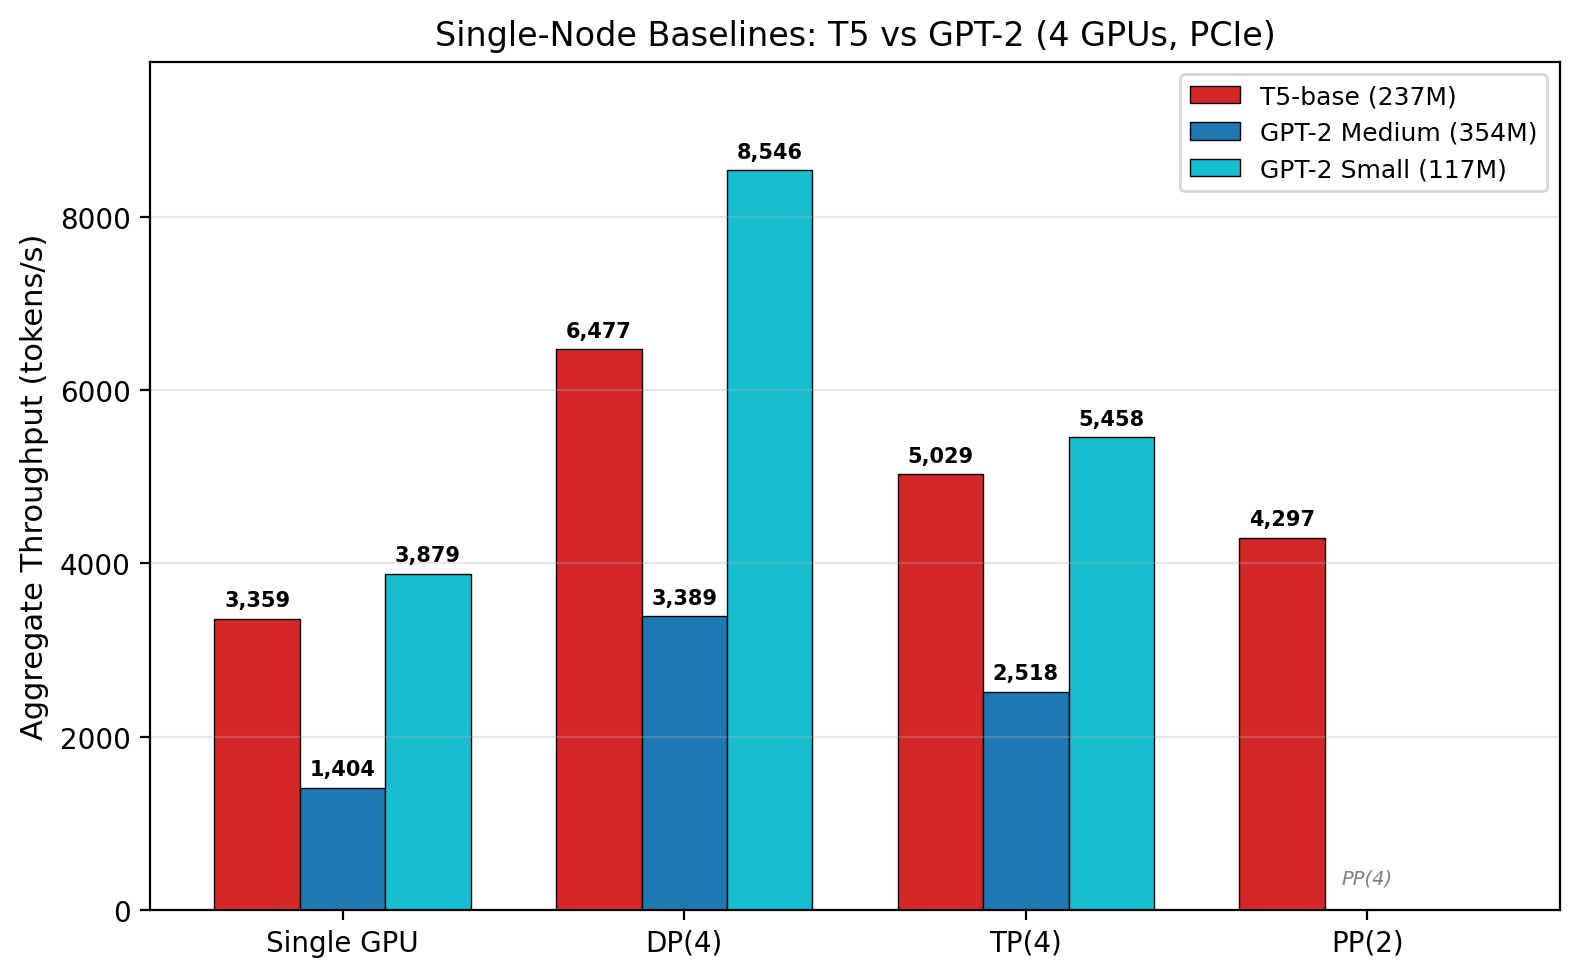
\includegraphics[width=\textwidth]{fig_phase3_t5_baselines.png}
  \end{column}
  \begin{column}{0.45\textwidth}
    \small
    \textbf{T5-base:} 12 enc + 12 dec layers, 237M params

    \vspace{0.3em}
    Two key differences from GPT-2:

    \vspace{0.2em}
    \textbf{1. Pipeline imbalance:}
    \begin{itemize}\small
      \item Encoder stage: 2.51 GB
      \item Decoder stage: 3.87 GB (\textbf{54\% heavier})
      \item Encoder idles waiting for decoder
    \end{itemize}

    \vspace{0.2em}
    \textbf{2. Extra TP communication:}
    \begin{itemize}\small
      \item Cross-attention $\rightarrow$ +1 all-reduce/block
      \item T5: \textbf{60} all-reduces/fwd pass
      \item GPT-2 Med: 48 all-reduces/fwd pass
      \item 25\% more communication
    \end{itemize}
  \end{column}
  \end{columns}
\end{frame}

% --- Slide 10: Architecture Scaling (Nadhiya) ---
\begin{frame}{Architecture Determines Scaling}
  \centering
  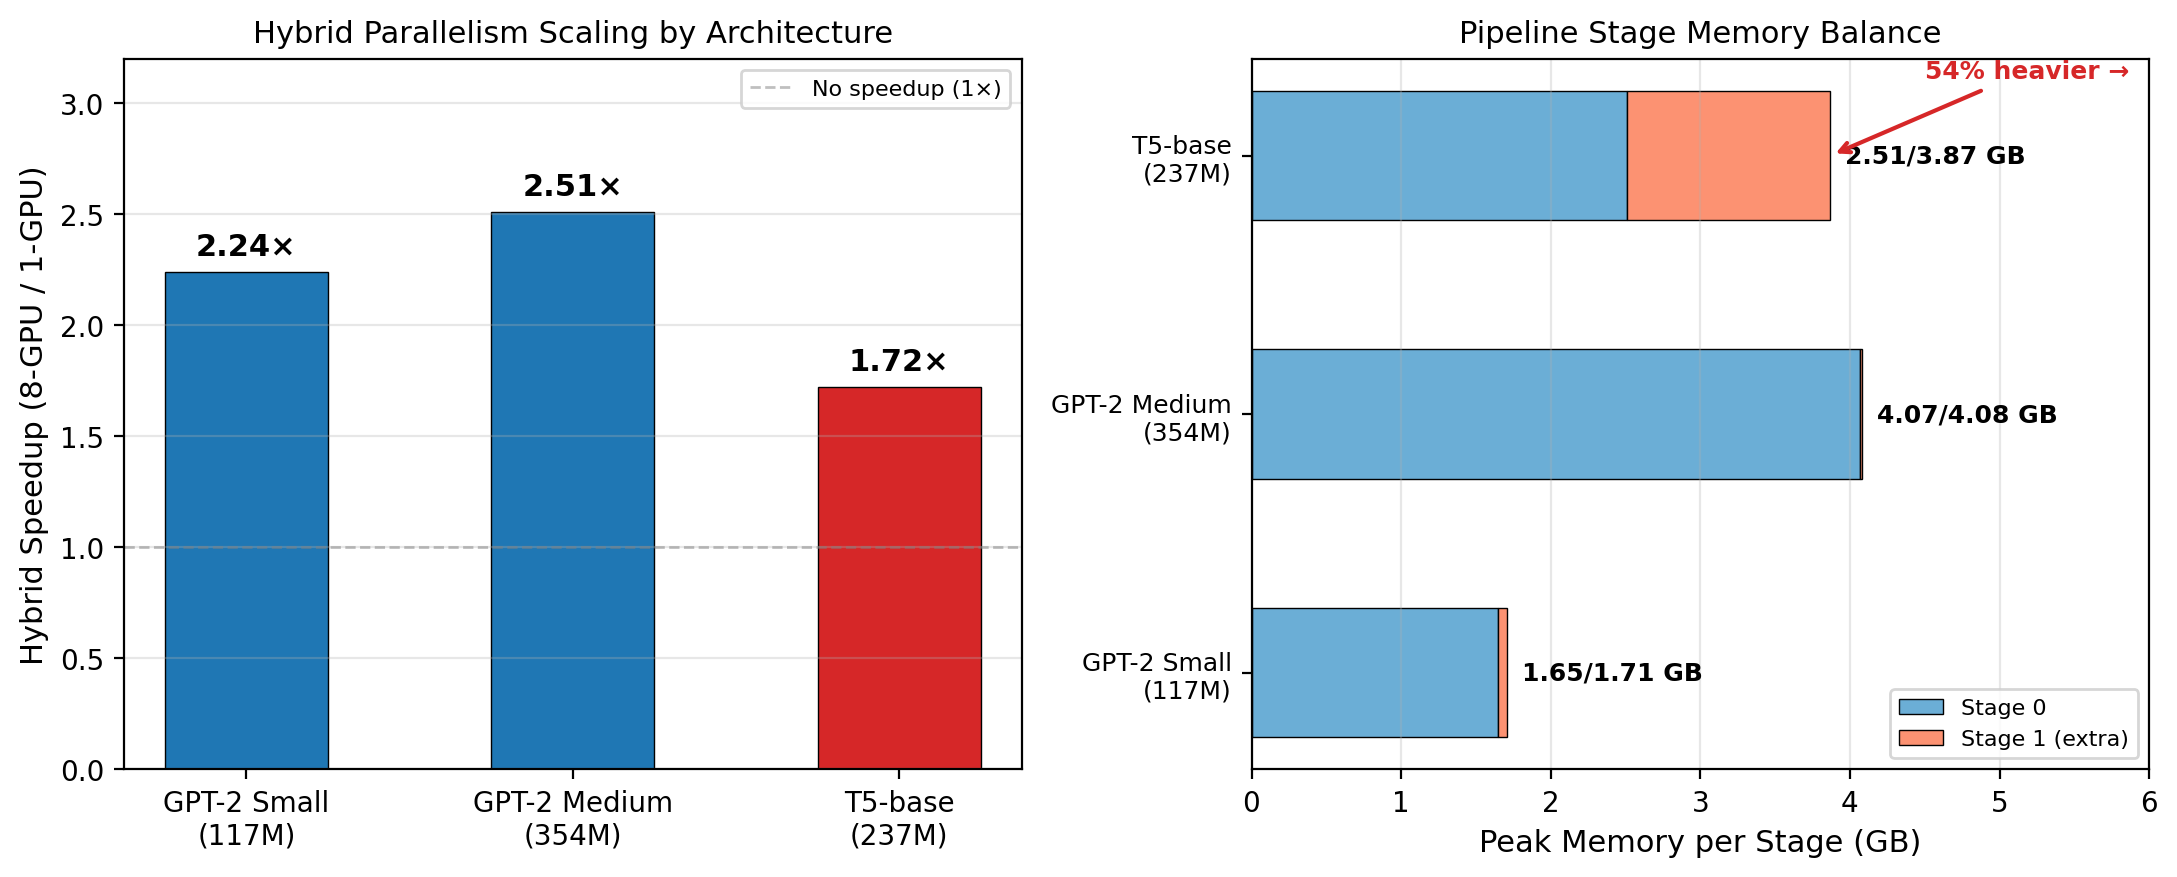
\includegraphics[width=0.75\textwidth]{fig_phase3_arch_scaling.png}

  \vspace{0.2em}
  \scriptsize
  \begin{tabular}{lrrrrl}
    \toprule
    \textbf{Model} & \textbf{Params} & \textbf{1-GPU} & \textbf{8-GPU} & \textbf{Speedup} & \textbf{PP Mem (S0/S1)} \\
    \midrule
    GPT-2 Small & 117M & 3,879 & 8,678 & \textbf{2.24$\times$} & 1.65 / 1.71 GB (balanced) \\
    GPT-2 Medium & 354M & 1,404 & 3,519 & \textbf{2.51$\times$} & 4.07 / 4.08 GB (balanced) \\
    T5-base & 237M & 3,359 & 5,790 & \textbf{1.72$\times$} & 2.51 / 3.87 GB (\textbf{54\% imbalance}) \\
    \bottomrule
  \end{tabular}

  \vspace{0.3em}
  GPT-2 Small (117M) is \textbf{smaller} than T5-base (237M) yet scales \textbf{better} (2.24$\times$ vs 1.72$\times$)\\
  $\Rightarrow$ The gap is \textbf{architectural}, not size-related.
\end{frame}

% ==================================================================
\section{Conclusion}
% ==================================================================

% --- Slide 11: Key Findings (Nadhiya) ---
\begin{frame}{Key Findings}
  \begin{enumerate}
    \item \textbf{Communication-aware placement matters:}\\
    Keeping DP+TP on the fast intra-node link delivers \textbf{17--27\% higher throughput} consistently across all models tested.

    \vspace{0.3em}
    \item \textbf{DP is the most placement-sensitive axis} (not TP):\\
    DP inter-node: 17--27\% penalty \quad|\quad TP inter-node at TP=2: $\sim$0\% penalty.\\
    DP gradient sync is bandwidth-bound ($\sim$1 GB+); TP messages are small at low degrees.

    \vspace{0.3em}
    \item \textbf{Placement effect is stronger for T5 (+27\%) than GPT-2 (+20\%):}\\
    T5's cross-attention gradients increase the DP synchronization volume.

    \vspace{0.3em}
    \item \textbf{Architecture determines hybrid parallelism scaling:}\\
    Symmetric GPT-2: 2.2--2.5$\times$ \quad|\quad Asymmetric T5: 1.72$\times$\\
    Due to pipeline imbalance (54\%) and 25\% more TP all-reduces from cross-attention.
  \end{enumerate}
\end{frame}

% --- Slide 12: Conclusion & Future Work (Nadhiya) ---
\begin{frame}{Conclusion \& Future Work}
  \textbf{Summary:}
  \begin{itemize}
    \item Built \textbf{Mini Colossal-AI}---4 parallelism strategies from scratch using \texttt{torch.distributed}
    \item Phase 2 (all-TCP): PP wins, TP/DP bottlenecked by network
    \item Phase 3 (PCIe + TCP): Communication-aware placement unlocks 3D hybrid parallelism
    \item Adding T5 reveals hybrid scaling benefits are \textbf{not universal}---they depend on architecture
    \item Validates placement heuristics used by Colossal-AI and Megatron-LM
  \end{itemize}

  \vspace{0.5em}
  \textbf{Future Work:}
  \begin{itemize}
    \item Sequence parallelism for long-context models
    \item Auto-tuning: select mesh dimensions given hardware topology
    \item Evaluation on NVLink + InfiniBand clusters
  \end{itemize}
\end{frame}

% ======== QUESTIONS ========
\begin{frame}
  \centering
  \vspace{2cm}
  {\Huge\bfseries Questions?}
  \vspace{1cm}

  {\large Dinesh Chand \quad Goutham P \quad Meena Chidambaram \quad Nadhiya R S}

  \vspace{0.3em}
  {\small MTech-AI, IISc Bangalore}
\end{frame}

\end{document}
